\documentclass[letterpaper]{article}
\usepackage{aaai19}
\usepackage{times} 
\usepackage{helvet}
\usepackage{courier} 
\usepackage[hyphens]{url}
\usepackage{graphicx}
\usepackage{float}
\urlstyle{rm}
\def\UrlFont{\rm}
\usepackage{graphicx}
\frenchspacing
\setlength{\pdfpagewidth}{8.5in}
\setlength{\pdfpageheight}{11in}
% custom packages%
\usepackage{amsmath}
\usepackage{enumitem}
\usepackage{subcaption}


\pdfinfo{
/Title (Measuring the Influence of Trollbots during the 2018 US Midterm Election)
/Author ()
}

\setcounter{secnumdepth}{2} %May be changed to 1 or 2 if section numbers are desired.

\title{Measuring the Influence of Trollbots in Twitter during the 2018 US Midterm Election}

\begin{document}

\maketitle

\begin{abstract}
    The use of troll bots in social media and its consequences has been a subject of great public interest. In this study, 
    we measure the influence of trollbots during 
    the 2018 US Midterm Elections. We selected 2.94M tweets and 870k 
    profile data posted between October 31, 2018, and November 7 using nine keywords. On December 10, 2019, 
    we rescraped Twitter to find suspended and removed accounts. We identified the suspended accounts 
    as Trollbots and used Machine Learning on the removed 
    accounts to find other trollbots. We found that the top 1\% of the Trollbots, influenced the creation of 7\% of all the tweets.
    In Twitter, Tweet or a retweet made by another user can be retweeted.
    We estimate the number of times the tweet or the retweet 
    gets retweeted by other users to calculate the influence of a Tweet.
    We added the influence of all Tweets made by a user to calculate user wise influence.\end{abstract}

\section{Introduction}
\label{sec:introduction}

Twitter is a social networking service where users interact with each other using short messages called Tweet. 
Tweets spread through retweets or replies. For example, when Alice replies/retweets, a tweet made 
by Bob, Alice and Bob's followers see the tweet. \par

People use social media, at least in part, to form an opinion about lifestyle, health, politics, and purchase 
\cite{varol2017early}. To reach many audience, various ethical and unethical 
techniques have been devised. 
One such unethical technique is the use of trollbots. Here we defined Trollbots as the account which violates
Twitter's terms of service. The most common reason for the suspension is spam and abusive behaviour 
\cite{twitter}. \par

In this study, we rely on Twitter for most of the bot detection to focus on measuring the influence.

\subsection{Summary and Findings}

\begin{itemize}
    \item 13.6\% of the users in the datasets no longer existed. 4.1\% had been suspended. Of the remaining 9.5\%, 22\% were bots. Overall, 6.19\% of the users were bots. They made 
    12\% of all the Tweets.
    \item On Average, trollbots were 53\% more influential than humans
    \item Top 1\% of the trollbots influenced the creation of 7\% of all the retweets/replies.
    \item On average, a single URL was shared 26.48 times in 1.98 cascades. When a Tweet 
    mentions a URL. Any further retweet belongs to the same cascade.
    \item For URLs that were shared more than ten times, the influence percentage of bots was 70\% greater than their 
    size.
    \item 74.18\% of all interaction (retweets and replies) took place between humans, and 1.78\% took place between 
    bots. 12.04\% was bot-human, and 12\% was human-bot interaction.
\end{itemize}
   
\section{Related Work}
\label{sec:related}

\subsection{Social Media, Trolls and Bots}
People are spending more and more time on social media. Globally, people spend 2 hours and 23 minutes on average in Social Media. 40\%  people use social media to stay up to date 
with news and current events \cite{2019_social_flagship_report}. 68\% of American adults get their news from
social media while 42\% find news on social media to be mostly accurate \cite{pew_research_news}.\par

12\% of US adults get news from Twitter\cite{pew_research_news}. Twitter is the number one platform for government 
leaders. 97\% of all UN members have an official presence in Twitter \cite{twiplomacy}. Furthermore, Twitter API 
provides easy access to data. Consequently, Twitter has been widely studied \cite{rizoiu2018debatenight,grinberg2019fake,bovet2019influence,morstatter2018alt,munger2017don,gruzd2014investigating,zannettou2019characterizing,howard2016bots}.
\par

Social Media have been used for positives like democratizing online discussion, organizing civil movements \cite{gonzalez2013broadcasters}, augumenting public health 
\cite{dredze2012social}, forecasting \cite{asur2010predicting,nguyen2015sentiment,liu2016predicting}, forming social connections \cite{ellison2007benefits}, and 
for other greater goods \cite{moorhead2013new,househ2014empowering}. However, recently, more focus is being put on the negatives with high focus on disinformation and bots
\cite{forelle2015political,bradshaw2017troops,marwick2017media}. \par

Different types of bots exist in social media. A simple bot will post predetermined messages at predetermined intervals \cite{haustein2016tweets}. Bots are also used to increase followers
and make an account appear popular \cite{cresci2015fame}. Here, Botnet refers to a network of social media bots working together to make an influence. Many botnets use 
a hybrid human/automation approach \cite{grimme2018changing}. Botnets have been used to promote spam \cite{ferrara2018measuring}, which seem to shifted to social media due to the effectiveness of spam filter \cite{gao2010detecting,chu2012detecting,ferrara2018measuring}, 
manipulate stocks \cite{ferrara2015manipulation}, manipulate elections \cite{morstatter2018alt}, 
and for various other purposes \cite{abokhodair2015dissecting}. Many of the suspended users are a part of Botnets.
Botnets were detected as early as 2010 US Midterm Election \cite{mitter2014categorization}. Over time, their use and
 study have increased. Studies have detected and analyzed bots in the 2017 German Federal Election \cite{morstatter2018alt} ,2017 French Presidential Election \cite{ferrara2017disinformation} and during 
various US Elections \cite{mitter2014categorization,bovet2019influence,rizoiu2018debatenight,bessi2016social,howard2018algorithms,howard2016bots,deb2019perils}. In Elections, 
they have been used to support candidates \cite{luceri2019red}, attack people \cite{mueller_investigation} and spread fake news \cite{vosoughi2018spread,grinberg2019fake}. 
Political bots are active beyond the election time. \cite{stewart2018examining} found that Russian bots infiltrated both right and left-leaning communities and spread different narratives 
\cite{mueller_investigation}. \par

In Twitter, the trollbots share content 
in multiple channels \cite{paul2016russian}. This activity is in line with literature, which shows that information 
from multiple sources appears more trustworthy than a single one \cite{harkins1981multiple}. 
 Trollbots attack people. Attacking trustworthiness has been shown to diminish the credibility of the Original Poster \cite{pornpitakpan2004persuasiveness}. 
Bots are continuous, repetitive, but most of the time, they are also far from reality \cite{paul2016russian}. 
The high volume seems to ensure early exposure and \cite{petty1994think} shows that early
 first impression is more likely to be accepted by the brain. Due to a phenomenon called Sleeper Effect, where information gets disassociated from the source while remembering \cite{underwood1998memory,paul2016russian}
 low credibility sources can have the persuasive power to unbiased or neutral people. As a boost to sleeper effect, people are 31\% more likely to remember what they see on twitter, 
 compared to the normal web \cite{twitter_remember}. \par

\subsection{Trollbot Detection}
Most studies \cite{rizoiu2018debatenight,yang2019arming,shao2018spread} use Botometer\cite{davis2016botornot,yang2019arming} for bot detection.
Botometer's Machine Learning algorithm provides an account-level bot classification. Botometer classifies account 
partially and completely automatized as bots. 
Botometer uses more than a thousand features created from temporal activity, network structure, content analysis, sentiment analysis, and user profile data to
determine a bot score \cite{davis2016botornot,yang2019arming}. \cite{bessi2016social} illustrated that profile 
customization, geographical metadata, and activity statistics provided the strongest signals for bot detection.
However, Botometer has high false positive and detects organizational accounts as bots \cite{varol2017early} \cite{botometer_tweet}.
\par

\cite{ferrara2017disinformation} and \cite{kudugunta2018deep} had success detecting bots using fewer features. 
\cite{ferrara2017disinformation} obtained 93\% accuracy with an AUC-ROC score of 92\% in their best model 
using Random Forest classifier. \cite{kudugunta2018deep} used 3,000 labelled examples to train a system with an 
AUC greater than 99\% using Adaboost Classifier with Over Sampling and Undersampling of data using the SMOTENN 
algorithm. \par

\subsection{Influence Detection}
\cite{zannettou2019let} uses Hawkes Process to determine the influence Iranian and Russian bots had on pushing URLs
 in 4 social media platforms. They found that Russian trolls were extraordinarily 
influential and efficient in spreading URLs. \cite{shao2018spread} found that bots amplify URLs in early moments 
before an article goes viral, while \cite{ferrara2018measuring} 
found the same for spam. Bots target users with many followers through replies and manipulation. This method was
 very efficient. \par


\cite{shao2018spread} found that articles spread 
mostly through tweets and retweets. Their study showed that people do not discriminate between resources 
shared by humans and bots. \cite{shao2018spread} and \cite{grinberg2019fake} found super spreaders. 
Moreover, \cite{grinberg2019fake} found that 1\% of individuals accounted for 80\% of fake news exposure. 
\cite{varol2017early} also found that 2\% user accounts were responsible for 60\% of the conversation. \par

\cite{rizoiu2018debatenight} found that social bots were 2.5 times more influential than humans. They used 
Botometer to label the bots and introduced a 
scalable algorithm for estimating user influence in retweet cascades. 
For each tweet in an information cascade, it uses time of post and the number of followers to determine the 
probability of whether a tweet is a retweet of another. They then find influence which can be used 
to find out how many users the tweet possibly influenced to retweet. It was tested successfully in 
artificial social media. Other studies have attempted to measure influence before this. 
\cite{weng2010twitterrank} used eigenvector centrality of the connection to measure influence, but it is 
not scalable into big cascades. There are other methods like 
\cite{rodriguez2011uncovering,cho2013latent,linderman2014discovering}, but they either have scaling issues or 
require a full diffusion graph, which Twitter does not provide.

\section{Methods}
\label{sec:method}
\subsection{Data Collection}
Tweets containing nine manually identified keywords were selected from collected live data from Twitter. The 
keywords are:

\begin{itemize}
    \item 2018Midterms
    \item Election
    \item Election2018
    \item 2018Senate
    \item WinBlue
    \item WinRed
    \item BlueWave
    \item RedWave
    \item Republican
    \item Democrat
\end{itemize}

Twitter provides Streaming API, Search API, and a premium Firehose API to give access to tweets. 
Streaming API provides limited access to live data, while Firehose API provides complete data. However, due to the 
associated costs, Firehose API was not an option in this study. \cite{morstatter2013sample} compares the 
Streaming API with Firehose API. They found that Streaming API was nearly as good as a random sample of Firehose API 
when the dataset was large enough. Although the 1\% API was not as good as a 1\% random sample from the Firehose API 
in all of their tests, it estimated the top hashtags correctly when the data was large enough. \par 

In this study, we use Streaming API. While collecting data, information about the tweeter and the tweet was collected. 

We collected following information about a tweet:
\begin{enumerate}[label=\textbf{\arabic*}]
    \item \textbf{Timestamp:} UTC Timestamp in which the post was made
    \item \textbf{ID:} Post ID provided by twitter
    \item \textbf{Text:} Text in the tweet and the parent tweet if the tweet is a reply
    \item \textbf{User:} Username of the tweeter/retweeter/replier
    \item \textbf{Replies:} The number of replies the tweet has received. During live collection, this value is zero. We collect them during recollection of top tweets.
    \item \textbf{Retweets:} The number of retweets the tweet has received. During live collection, this value is zero. We collect them during recollection of top tweets.
    \item \textbf{Likes:} The number of likes the tweet has received. During live collection, this value is zero. We collect them during recollection of top tweets.
    \item \textbf{Reply To ID:} The ID of the parents tweet if this is retweet or a reply.
    \item \textbf{Response Type:} Either Tweet or Retweet or Reply
\end{enumerate}
\bigskip

We collected the following profile information from the Twitter API:
\begin{enumerate}[label=\textbf{\arabic*}]
    \item \textbf{Username:} Username of the user who posted the tweet
    \item \textbf{Location:} Binary if geolocation is enabled
    \item \textbf{Is Verified:} A binary if the profile has been verified
    \item \textbf{Total Tweets:} Total number of tweets created by the user
    \item \textbf{Total Following:} Total accounts the user is following
    \item \textbf{Total Followers:} Total Followers
    \item \textbf{Total Listed:} Number of times a user has been listed
    \item \textbf{Total Status:} Total Status
    \item \textbf{Total Likes:} Total likes the user has received
    \item \textbf{Has Background:}  Binary if an account has a background
    \item \textbf{Is Protected:}  Binary if an account is protected
    \item \textbf{Profile Modified:}  Binary if a profile has been modified
\end{enumerate}
\bigskip
\cite{kudugunta2018deep} and \cite{ferrara2017disinformation} use the same parameters in their machine learning 
architecture. \par

We collected Tweets from October 31, 2018 (1 AM UTC) to November 7, 2018 (midnight UTC). On July 18, 2019, we used 
Twitter API to rescrape the top 100k most retweeted Tweets which did not exist in our dataset.

\subsection{Data Processing}
We used SentiStrength in the Tweets to compare the sentiment. SentiStrength \cite{thelwall2010sentiment} is used 
to annotate short, informal tweet like texts \cite{bessi2016social}. 
It can capture positive and negative emotions at an accuracy of 60.6\% and 72.8\%. SentiStrength gives a positive 
and negative score between 0 and 4. The positive sentiment is subtracted from the negative like in \cite{bessi2016social} to get a whole number. SentiStrength is used instead of another 
popular solution VADER because it performed better in manual analysis.

\subsection{Trollbot Detection}
A year after the data collection, we checked twitter to find accounts that no longer existed. 117650 of the 863539
accounts did not. Of them, the 32323 suspended accounts were verified to be troll bots. The remaining 85327 
could or could not be bots as they also include accounts deactivated by users. So, we used Machine Learning in this 
data. Initially, we had used Machine Learning on the complete dataset, but we received bad accuracy using that 
mechanism. \par

We selected 95\% of suspended users and an equal amount of random non suspended users, which we conveniently refer to as humans to train a SMOTENN network using 
the profile features detailed above. It had an AUC of 0.95 in the training set and 0.93 in the test set.


\subsection{Cascading and Influence Detection}
A tweet cascade starts when a Tweet is made. Any retweet or response which involve that Tweet belongs to that cascade. If Bob retweets Alice's tweet, and Eve retweets Bob's retweet, the tweets
made by Alice, Bob, and Eve will belong in the same cascade. The Twitter API will show Eve and Bob as a direct descendant of Alice without any mention that Eve retweeted Bob's retweet. \par

\cite{du2013scalable} defines influence as the average number of users who get in contact with the content created by a user \textit{u}.
 However, Twitter does not provide the diffusion graph and the number of people reached. \cite{rizoiu2018debatenight}
  define the influence of a user over a retweet cascade as "the expected number of time the tweet is
 retweeted – direct retweets or descendants in a diffusion scenario – over all possible diffusion scenarios  
 associated." They define the influence of a user as the sum of the influence of tweets
 authored by a user. We use their algorithm and definition. \cite{rizoiu2018debatenight} uses time and 
 number of followers to estimate a user influence. Using this mechanism, a high influence score can be provided to highly connected users who never start diffusions and 
 to active retweeters with little followership. \cite{rizoiu2018debatenight} tested their algorithm on an artificial social network with 1000 users and found that the influence calculated had a Spearman 
 correlation coefficient of 0.88 with the actual influence. \par 

In \cite{rizoiu2018debatenight}'s algorithm, for each tweet in a cascade, the probability of it being a descendant of each previous tweet is calculated using a softmax function. Mathematically, probability that a \textit{j\textsubscript{th}} 
tweet is a retweet of \textit{i\textsubscript{th}} tweet is measured by :\linebreak

\begin{equation*}
    p_{ij}=\frac{{m_{i}e^{-r(t_j-t_i)}}}{\sum_{k=1}^{j-1}m_ke^{-r(t_j-t_k)}}
    \label{eq:probablity}
\end{equation*}

where, \par
\textit{t\textsubscript{j}{-}t\textsubscript{i}} is used as exponential decay between the timing of original tweet and that of the retweet, \par
\textit{r} is a hyperparmeter which they found to be $6.8\times10\textsuperscript{-4}$, \par
\textit{m} is the number of followers \linebreak

Then for every tweet in a cascade, pairwise influence is calculated as:

\begin{equation}
    m_{ij} =
      \begin{cases}
        \sum_{k=i}^{j-1}m_{ik}p_{kj}^2 & \text{,i \ \textless \ j}\\
        1 & \text{,i \ = \ j}\\
        0 & \text{,i \ \textgreater \ j}
      \end{cases}       
    \end{equation}

Then the total influence of a node is the sum of the pairwise influence score m\textsubscript{ij} over all subsequent nodes. For a derivation of this, the original study
 \cite{rizoiu2018debatenight} and its citations should be referred. \par

 \cite{rizoiu2018debatenight} tested the validation of their algorithm when they had access to full data. As we used streaming API, we did not. So random cascades were synthesized using the following algorithm 
 to test the validity:
 
 \begin{itemize}
    \item An aggregate database \textit{D} was created. In the database \textit{D}, values of \textit{D\textsubscript{u}} was set to all possible usernames  and \textit{D\textsubscript{u}\textsuperscript{a}}
     and \textit{D\textsubscript{u}\textsuperscript{s}} set to 0.
    \item For 500000 cascades, following steps was repeated:
    \setlength{\itemindent}{+.3in}
    \item Length of cascade, n was randomly selected from the all possible size of cascades we captured. Then n random values were selected from our cascade that included 
    username, time and followers count.
    \item Influence was calculated for the selected n values. 1\% of values were randomly selected from the n, and influence was calculated for it too.
    \item The total sample influence, \textit{D\textsubscript{u}\textsuperscript{s}} and actual influence \textit{D\textsubscript{u}\textsuperscript{a}} in the dataset D was updated for a user u,
    by adding the calculated value with the current values of \textit{D\textsubscript{u}\textsuperscript{s}} and \textit{D\textsubscript{u}\textsuperscript{a}}.
 \end{itemize}

Then we converted the raw influence score to a user wise percentage. A correlation of 0.96 existed between the full dataset and the 1\% sample. We used this method 
 instead of \cite{rizoiu2018debatenight}'s original one due to limitations in computing power.


 \section{Data Analysis}
\label{sec:analysis}

\subsection{Exploratory Data Analysis}
Our dataset consisted of 2.94M Tweets by 870k users. After Machine Learning, 6.19\% of these accounts 
were found to be bots. They made 15.6\% of the Tweets. The mean 
sentiment of bots was -0.19, slightly more negative than the average non-bot at -0.16. We 
removed stopwords to compare the words used by bots and humans (used for convenience to refer to users who are not Trollbots). 
We selected words that appear more than 0.03\% times in the dataset (which was 41386 times for humans and 6148 for 
bots). The dominant words are in 
\ref{tab:bot-dominant-words} and \ref{tab:humans-dominant-words}. From Table \ref{tab:bot-dominant-words}, 
we can see that most of the trollbots seem to be alt-right or republican. Qanon is an alt-right conspiracy theory 
while kag refers to "Keep America Great". Other bot dominant words are also popular among the republicans.
Among humans, one incident seems to have stood out. A Florida State University (FSU) student had been 
arrested for throwing chocolate milk and the word related to it dominate the human side.

\begin{table}[h]
    \begin{tabular}{|l|l|}
    \hline
    \textbf{Word} & \textbf{\begin{tabular}[c]{@{}l@{}}Percentage\\ Difference\end{tabular}} \\ \hline
    chocolate     & 78.885052                                                                \\ \hline
    milk          & 76.540881                                                                \\ \hline
    fsu           & 76.08353                                                                 \\ \hline
    throwing      & 75.873016                                                                \\ \hline
    woman         & 59.52                                                                    \\ \hline
    arrested      & 58.247903                                                                \\ \hline
    men           & 56.640345                                                                \\ \hline
    jewish        & 55.259654                                                                \\ \hline
    nazis         & 49.34877                                                                 \\ \hline
    name          & 46.192053                                                                \\ \hline
    put           & 44.897959                                                                \\ \hline
    away          & 43.264503                                                                \\ \hline
    something     & 41.046607                                                                \\ \hline
    angry         & 40.981013                                                                \\ \hline
    think         & 40.675676                                                                \\ \hline
    \end{tabular}
    \caption{Words used more often by humans}
    \label{tab:humans-dominant-words}
\end{table}

\begin{table}[h]
    \begin{tabular}{|l|l|}
    \hline
    \textbf{Word}        & \textbf{percentage\_difference} \\ \hline
    qanon                & 32.315522                       \\ \hline
    kag                  & 31.95122                        \\ \hline
    walkaway             & 28.093948                       \\ \hline
    usa                  & 27.511962                       \\ \hline
    patriots             & 26.732673                       \\ \hline
    racism               & 26.315789                       \\ \hline
    lie                  & 25.85034                        \\ \hline
    americafirst         & 25.561798                       \\ \hline
    wwg1wga              & 25.519288                       \\ \hline
    voteredtosaveamerica & 25.504152                       \\ \hline
    low                  & 24.262295                       \\ \hline
    truth                & 24.08377                        \\ \hline
    borders              & 23.773006                       \\ \hline
    destroy              & 23.054755                       \\ \hline
    lying                & 22.685185                       \\ \hline
\end{tabular}
\caption{Words used more often by bots}
\label{tab:bot-dominant-words}
\end{table}

Then we analyzed the 141436 cascades containing more than ten tweets to calculate human-bot interaction. 
We made the following observations: 

\begin{itemize}
    \item 1.78\% of all retweets were made from bot Tweets by bots.
    \item 12.04\% of all retweets were made from bot Tweets by humans.
    \item 12\% of all retweets were made from humans Tweets by bots.
    \item 74.18\% of all retweets were made from human Tweets by humans.
\end{itemize}

\begin{figure}[H]
    \centering
    \begin{subfigure}[b]{1\linewidth}
      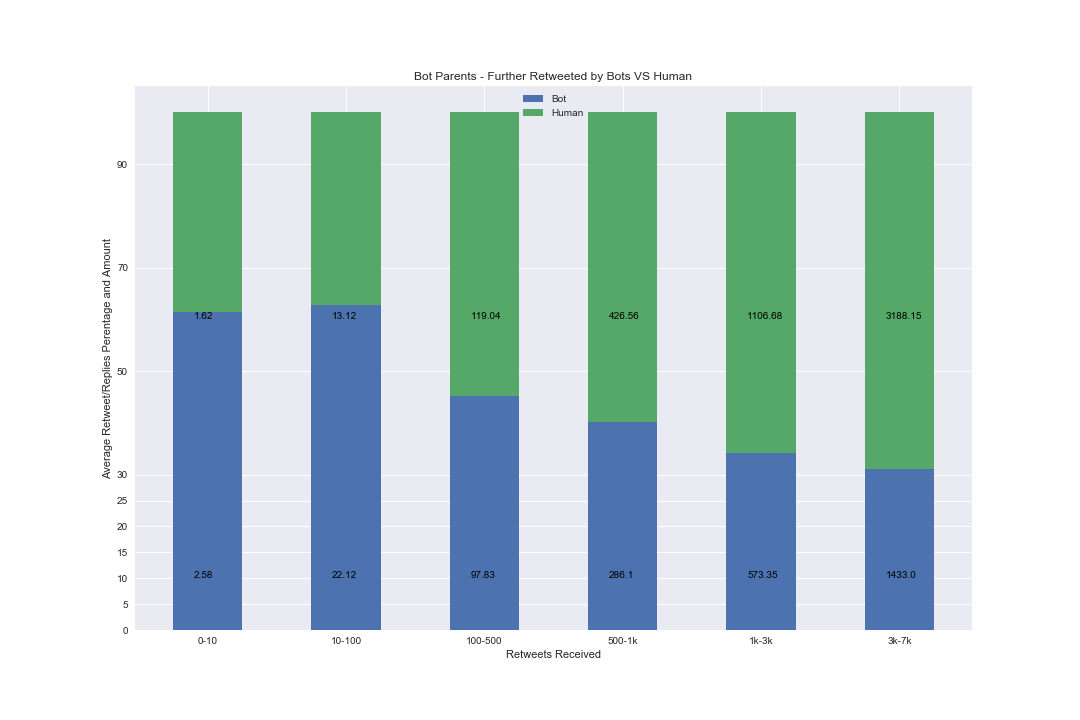
\includegraphics[width=\linewidth]{images/bots_furtherretweeted.png}
      \caption{Bots Parents}
      \label{fig:further_retweet_bots}
    \end{subfigure}
    \begin{subfigure}[b]{1\linewidth}
      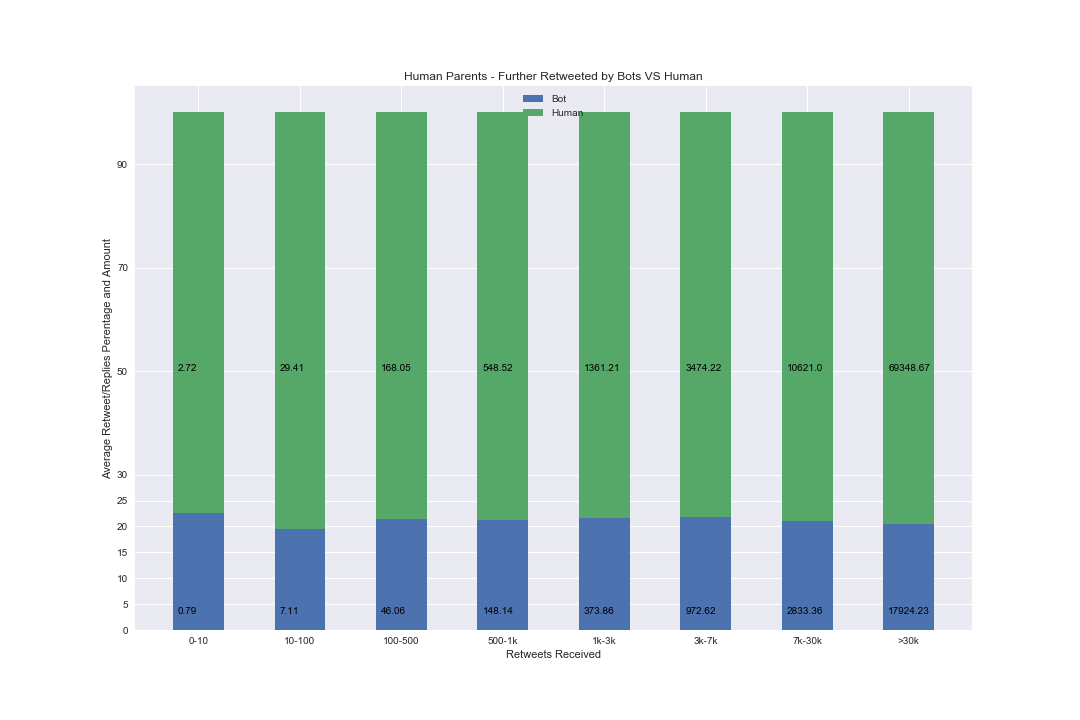
\includegraphics[width=\linewidth]{images/humans_furtherretweeted.png}
      \caption{Humans Parents}
      \label{fig:further_retweet_humans}
    \end{subfigure}
    \caption{Retweet cascades for tweets made by humans and bots are grouped by their size and visualized. Here, we see 
    that bots dominate cascades started by bots in the early retweets. As the size gets bigger, more humans see it. For 
    human started tweets, their percentage is similar in all sizes}
    \label{fig:further_retweet}
\end{figure}

Next, we compared the cascades started by bots and humans. Figure \ref{fig:further_retweet} can be zoomed 
for detail. In Figure \ref{fig:further_retweet_bots} we can see that the percentage of bots was high for smaller cascades 
started by bots. As the size of the cascade increases, the percentage of bots decreases. 
We made the opposite observation for humans in Figure \ref{fig:further_retweet_humans}. If a tweet receives 
few audiences, they are the followers. Bots are mostly
followed by bots and humans by humans. This finding goes in line with those made by earlier research which
 shows that bots and humans are mostly followed by their type. \par

\subsection{Retweet Influence Analysis}

The average influence of a human was 4.12, while that of a trollbot was 6.34. This is lesser than 
\cite{rizoiu2018debatenight}'s finding who found that bots were 2.5 times more influential than humans. 
But they used Botometer to determine bots while we relied mostly on Twitter.

Figure \ref{fig:humans_bots_percentage} shows the most influential users. 

\par

\begin{figure}[H]
    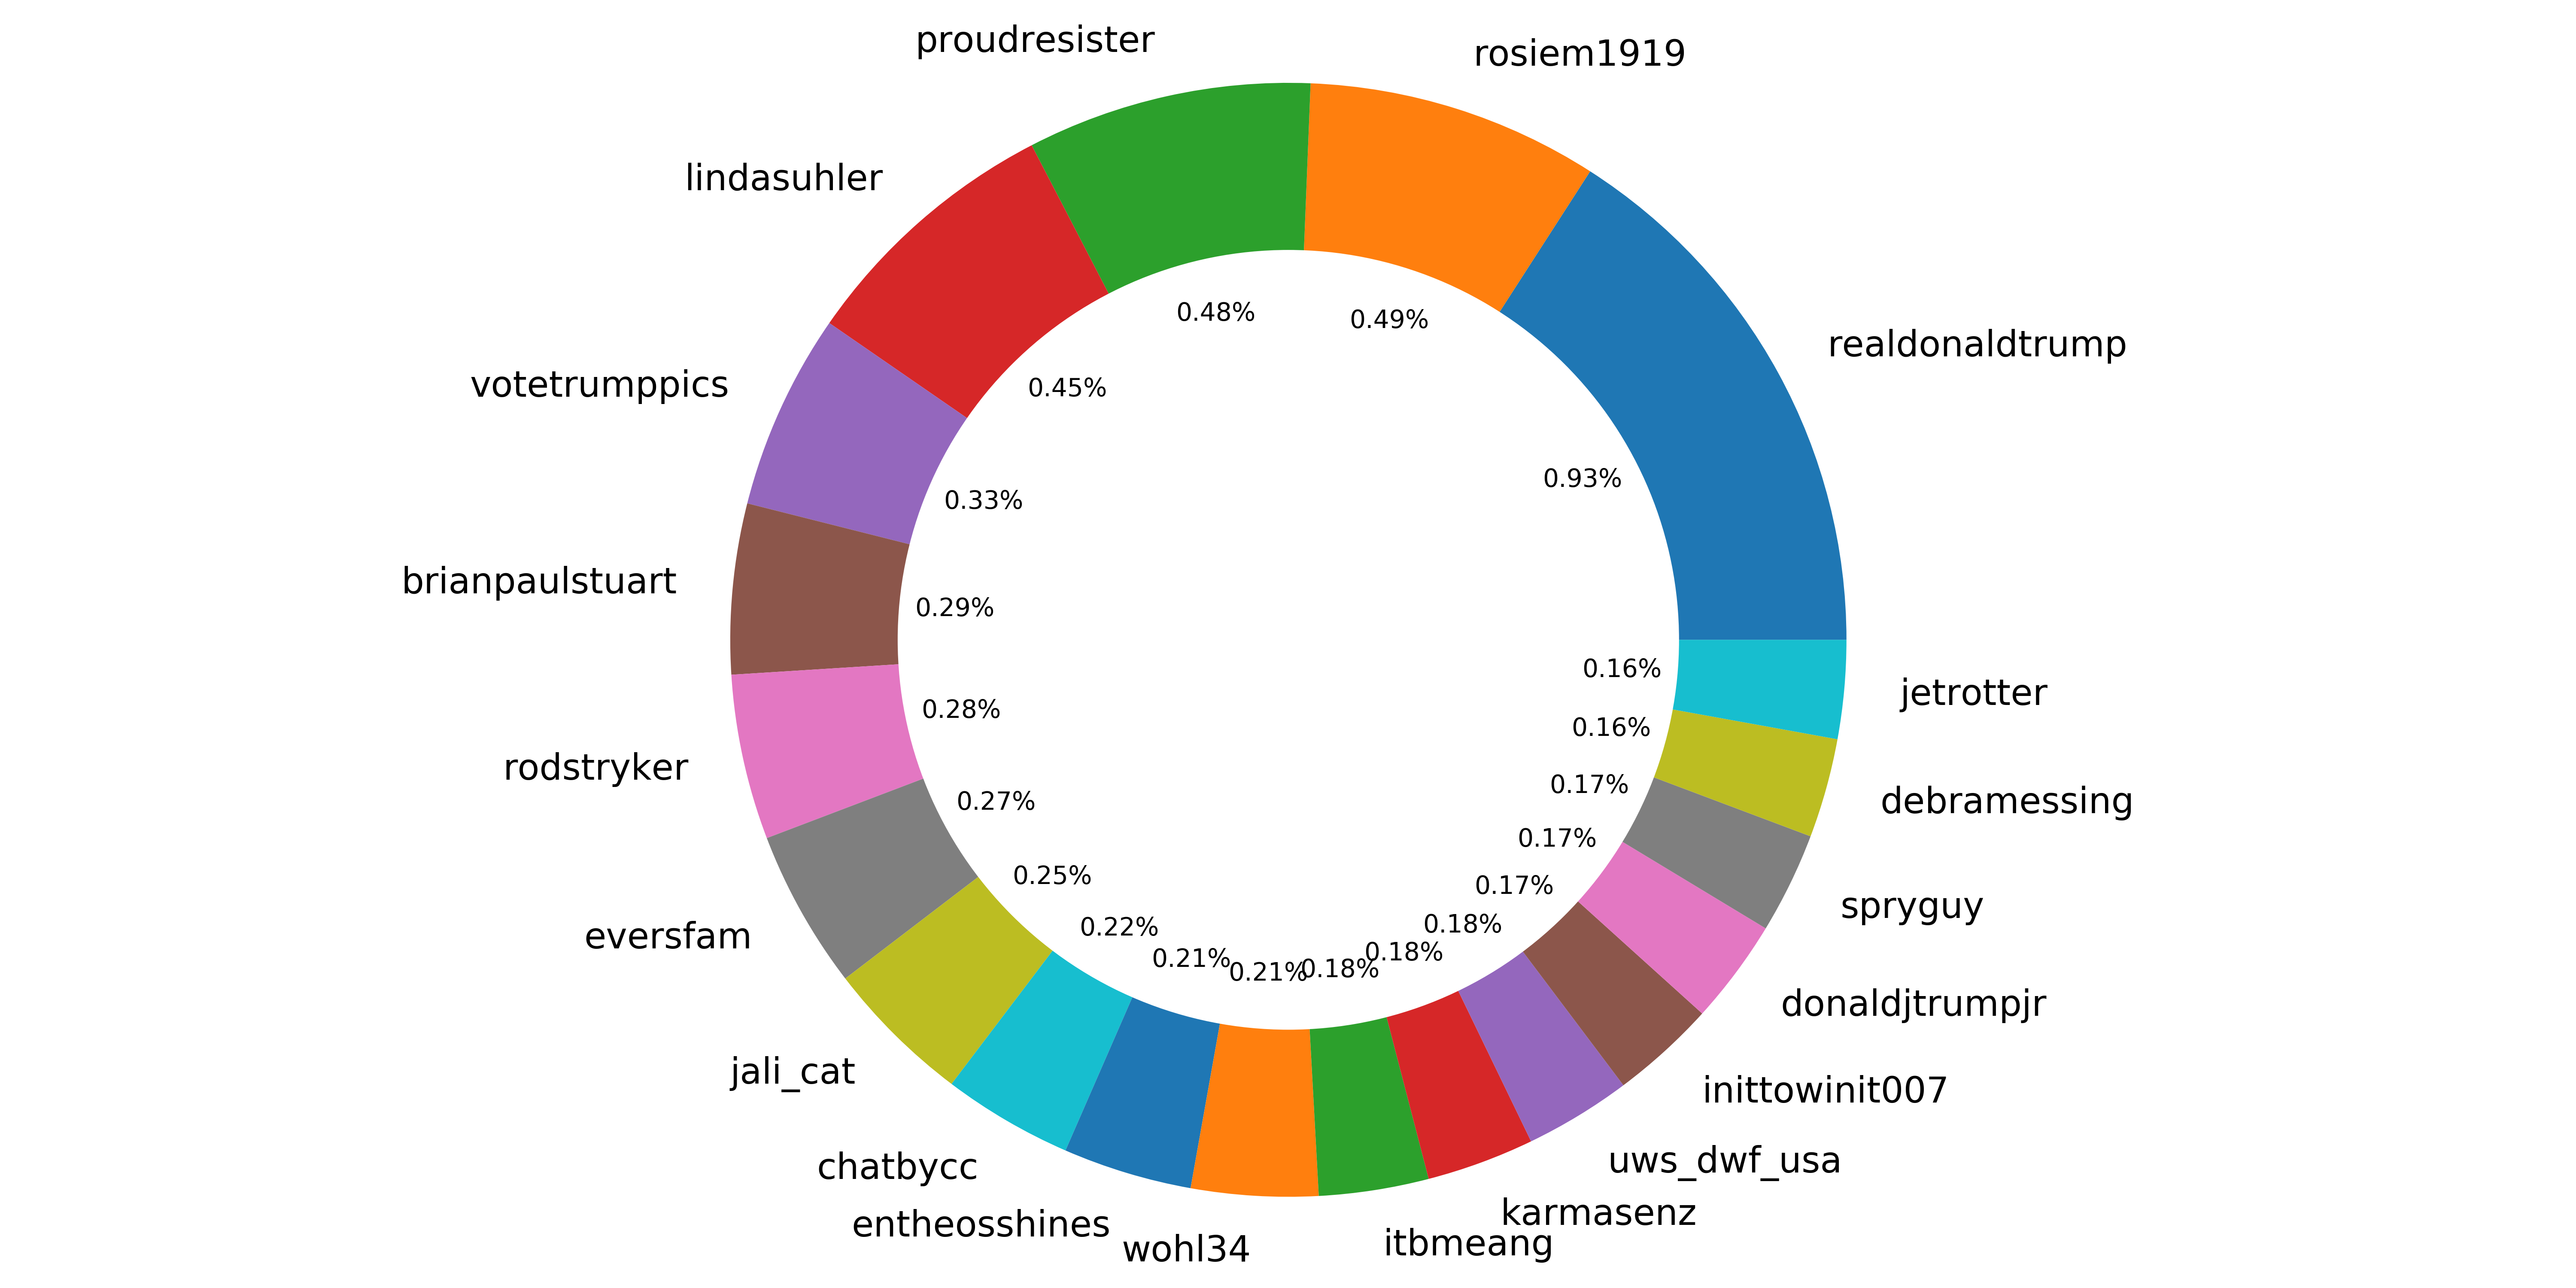
\includegraphics[width=\linewidth]{images/top_influences.png}
    \caption{Most influential users. Users with many followers and users who made many tweets were found to be the most influential ones. Most interesting is user @swtwrwfwrw who made over 500 tweets during this timeframe and was found to be more influential than @DonaldJTrump}
    \label{fig:humans_bots_percentage}
\end{figure}

Then, we measure made by the percentage of users. To find this out, we first calculated the user wise 
influence of all users in our dataset as a sum of their influence in all their tweets. Then, we used our 
label bots and not bots, referred conveniently as humans. We calculated the Influence
 percentage by using the total influence of all users. Figure \ref{fig:top_infuence}, shows that 
that in both categories top 1\% of the users account for around 70\% of their total influence \par

\begin{figure}[H]
    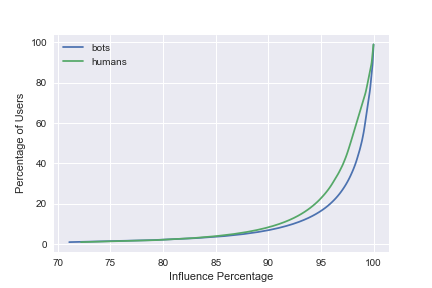
\includegraphics[width=\linewidth]{images/top_percentages.png}
    \caption{Percentage of top users and their influence percentage.}
    \label{fig:top_infuence}
\end{figure}

Bots are responsible for 10\% of the total influence, while the top 1\% is responsible for 7\%. 
Out of 2.94M data in our cascade, this might imply 
that bots were responsible for the creation of 180k human tweets. However, we cannot make this conclusion 
without further research. When calculating influence, we could have calculated the influence of a bot or a
 human in the diffusion graph multiple times. We use the graph in \ref{fig:diff_graph} to illustrate 
the problem in making this assumption.

\begin{figure}[H]
    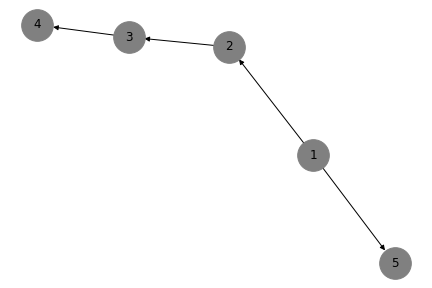
\includegraphics[width=\linewidth]{images/diffusion_graph.png}
    \caption{Diffusion Graph}
    \label{fig:diff_graph}
\end{figure}

In Figure \ref{fig:diff_graph}, the influence score of node 1 will be 4, node 2 will be 2, of node 3 will be 1, and of node 4 and node 5 will be 0. If 1 and 2 are bots, 
the total bot influence score will be 6. However,1 created 
2. Although this disparity might cancel out in 2 large groups across a large dataset when taken in percentage, we still refrain from making that conclusion. 
Further research is needed to make 
this verification. If we can make the verification, we can measure the impact of bots in terms of monetary value by comparing it with the advertising cost.

\subsection{URL Influence Analysis}
Before performing URL influence calculation, we resolved short URLs and removed twitter.com links. We kept the URLs 
which we could not resolve as they were. 
217,350 unique URLs belonging to 53,378 unique domains were shared in our dataset by 210,102 unique users 0.6 Million
times. Ten most popular domains in our dataset with their frequency are
in Table \ref{tab:Common_urls}. The top 10 domains for humans and bots, apart from t.co are in Table 
\ref{tab:common_human_bots}.

\begin{table}[H]
    \centering
    \begin{tabular}{|l|l|}
    \hline
    \textbf{Domain Name} & \textbf{Frequency} \\ \hline
    t.co & 127717 \\ \hline
    vote.gop & 96127 \\ \hline
    thehill.com & 57476 \\ \hline
    cnn.com & 54129 \\ \hline
    youtube.com & 51347 \\ \hline
    wtxl.com & 38124 \\ \hline
    nytimes.com & 35863 \\ \hline
    foxnews.com & 35277 \\ \hline
    instagram.com & 31634 \\ \hline
    breitbart.com & 30290 \\ \hline
    pscp.tv & 27702 \\ \hline
    \end{tabular}
    \caption{Most Common URLs}
    \label{tab:Common_urls}
\end{table}


\begin{table}[H]
    \centering
    \begin{tabular}{|l|l|}
    \hline
    \textbf{Human} & \textbf{Bots} \\ \hline
    vote.gop & vote.gop \\ \hline
    thehill.com & youtube.com \\ \hline
    cnn.com & foxnews.com \\ \hline
    youtube.com & breitbart.com \\ \hline
    wtxl.com & thegatewaypundit.com \\ \hline
    nytimes.com & pscp.tv \\ \hline
    foxnews.com & cnn.com \\ \hline
    instagram.com & instagram.com \\ \hline
    breitbart.com & thehill.com \\ \hline
    pscp.tv & facebook.com \\ \hline
    \end{tabular}
    \caption{Most Common Human and Bots URL}
    \label{tab:common_human_bots}
\end{table}

A single URL was shared 26.48 times in 1.98 cascades on average.

We found that the in URL cascades, for URLs that were shared more than ten times, the influence percentage of bots was 70\% greater than their size.

\section{Conclusion, Limitations and Further Work}
In this study, we show that bots have been highly influential and that most of the influence comes from a few top 
bots. In our dataset, 6.19\% of the users were bots. They created 12\% of the Tweets are their average influence was 
53\% more than that of a human. Overall they accounted for 10\% of the total influence, and the top 1\% were 
responsible for 7\% of the influence. In line with previous research, we have also shown that bots 
and humans form a cluster around each other and join when a tweet gets successful. This knowledge can help to point
 out a possible direction in the fight against bots. 

\begin{itemize}
    \item We performed this study in a limited dataset. It would have been better to perform it in the complete data. However, we did not have access to it. 
    Twitter Firehose API or Search API can be used in the future to have complete access to the data. Apart from Firehose and Search API, 
    a mechanism for finding Twitter posts using Twitter's snowflake algorithm looks promising \cite{bettermetrics2019}
    \item The current analysis was done by considering all bots as a single entity. Although easy, this distinction has many flaws. In futures, attempts should be made to 
    divide different types of bots and study their agenda
    \item As Twitter attracts some demographics more than others, using random Twitter data is not representative of the nation or the voting population. 
    Careful clustering can be done to create a representative data to get representative influence in the future.
    \item The validation of the influence detection algorithm can be done in a better way. Even Machine Learning techniques can be used to make a better influence detection algorithm 
    to predict the diffusion edges.
    \item Reddit can be analyzed along with Twitter to create a better spread graph. A bot detection system can be made for Reddit too. Combining multiple sources, a
     long term study can be conducted to measure the success/failure of bots in changing people's opinion.
\end{itemize}

\bibliographystyle{aaai}
\bibliography{references}

\end{document}